\section{Network Architecture}%
\label{subsec:l2hmc_network}
As previously mentioned, each of the functions $Q$, $S$, and $T$, are
implemented using multi-layer perceptrons with shared weights.
%
It's important to note that we keep separate the network responsible for
paramterizing the functions used in the position updates (`$\Xnet$', i.e.\
$Q_x$, $S_x$, and $T_x$), and the network responsible for parameterizing the
momentum updates (`$\Vnet$', i.e.\ $Q_v$, $S_v$, and $T_v$).
%
% Since both networks are identical, we describe the architecture of $\Vnet$
% below, and include a flowchart for $\Xnet$ illustrative purposes in
% Fig~\ref{fig:x_net_flowchart}.
%
\begin{figure}[htpb]
  \centering
  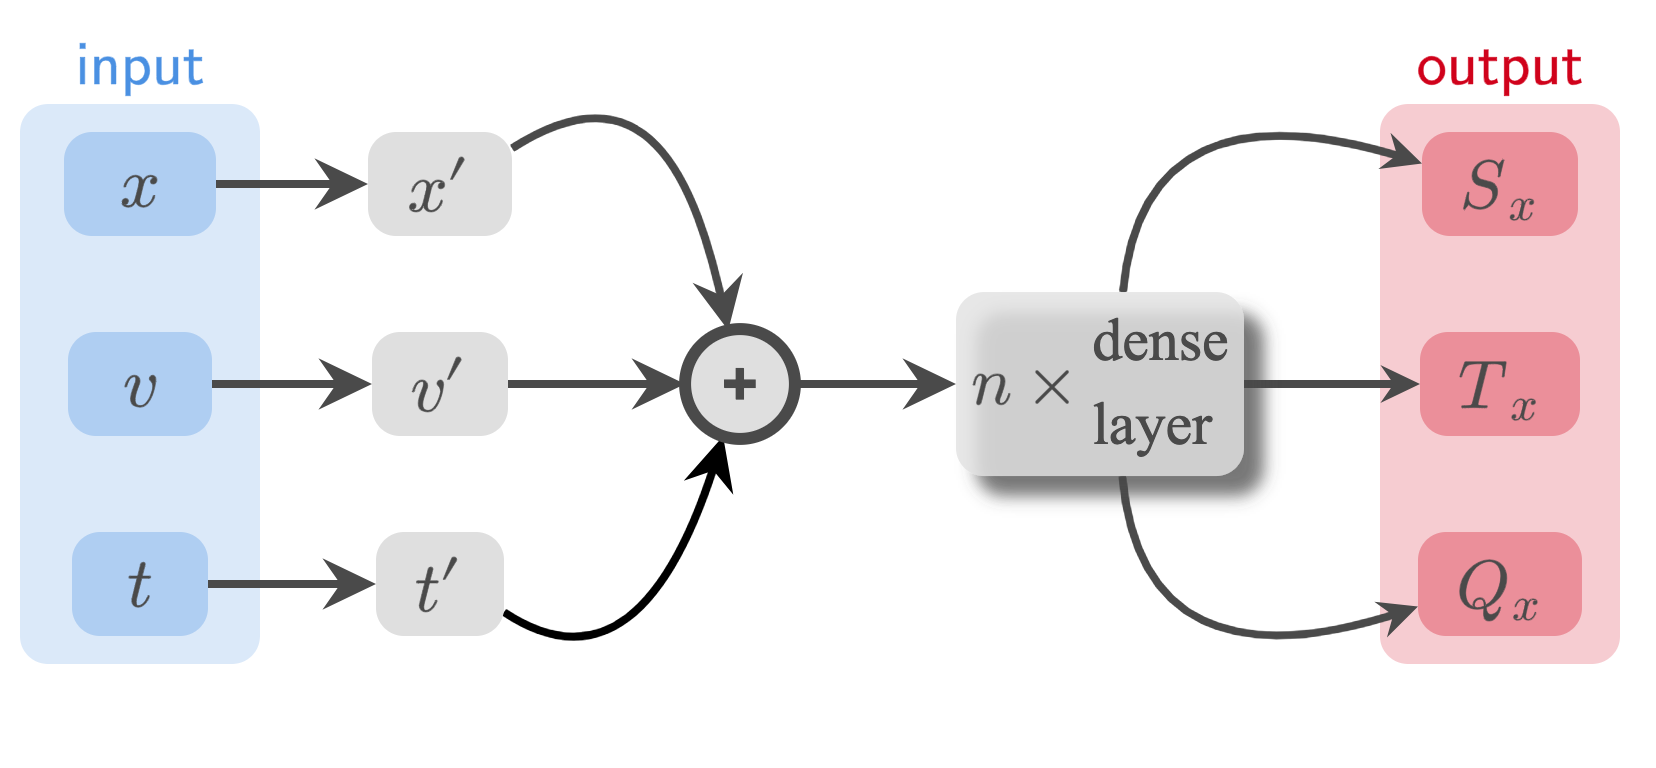
\includegraphics[width=\textwidth]{final/net.png}
  \caption{Illustration showing the generic (fully-connected) network
    architecture for training $S_x$, $Q_x$, and $T_x$.}%
    \label{fig:xnet}
\end{figure}

% \begin{figure}[htpb]
%   \centering
%   \input{tikz/vnet}
%   \caption{Illustration showing the generic (fully-connected) network
%     architecture for training $S_v$, $Q_v$, and $T_v$. Figure adapted
%     with permission from~\cite{joeyl2hmc}.}%
% \label{fig:generic_net}
% \end{figure}
%

The network takes as input $\zeta_1 = (x, \partial_{x} U(x), t)$, where $x, v
\in \mathbb{R}^{n}$, and $t$ is encoded as $\tau(t) = \left(\cos{(\frac{2\pi
t}{N_{\mathrm{LF}}})},\right.  \left.\sin{(\frac{2\pi
t}{N_{\mathrm{LF}}})}\right)$.
%
Each of the inputs is then passed through a fully-connected (`dense' layer),
consisting of $n_h$ hidden units
%
\begin{align}
    \tilde x &= W^{(x)} x + b^{(x)} \quad (\in \mathbb{R}^{n_h})\\
    \tilde v &= W^{(v)} v + b^{(v)} \quad (\in \mathbb{R}^{n_h})\\
    \tilde \tau &= W^{(\tau)} \tau + b^{(\tau)} \quad (\in \mathbb{R}^{n_h}).
\end{align}
%
Where $W^{(x)}, W^{(v)} \in \mathbb{R}^{n \times n_h}$, $W^{(t)} \in
\mathbb{R}^{2 \times n_h}$, and $b^{(x)}$, $b^{(v)}$,  $b^{(t)} \in
\mathbb{R}^{n_h}$.
%
From these, the network computes
%
\begin{equation}
    h_1 = \sigma(\tilde x + \tilde v + \tilde \tau) \quad (\in
    \mathbb{R}^{n_h}).
    \label{eq:hidden_1}
\end{equation}
%
Where $\sigma(x) = \max(0, x)$ denotes the rectified linear unit (ReLU)
activation function.
%
Next, the network computes
%
\begin{equation}
    h_2 = \sigma\left(W^{(h_1)} h_1 + b^{(h_1)}\right) \quad (\in
    \mathbb{R}^{n_h}).
    \label{eq:hidden_2}
\end{equation}
%
These weights ($h_2$) are then used to compute the network's output:
%
\begin{align}
    S_x &= \lambda_S \tanh(W^{(S)} h_2 + b^{(S)})\quad (\in \mathbb{R}^{n})\\
    Q_x &= \lambda_{Q} \tanh(W^{(Q)} h_2 + b^{(Q)})\quad (\in \mathbb{R}^{n})\\
    T_x &= W^{(T)} h_2 + b^{(T)}\quad (\in \mathbb{R}^{n}),
\end{align}
%
Where $W^{(s)}, W^{(q)}$, and $W^{(T)} \in \mathbb{R}^{n_h \times n}$ and
$b^{(s)}, b^{(q)}$, and $b^{(T)} \in \mathbb{R}^{n}$.
%
The parameters $\lambda_s$ and $\lambda_q$ are additional trainable variables
initialized to zero.
%
The network used for parameterizing the functions $T_v$, $Q_v$ and $S_v$ takes
as input $(x, \partial_x U(x), t)$ where again $t$ is encoded as above.  The
architecture of this network is the same, and produces outputs $T_v$, $Q_v$,
and $S_v$.

% \begin{figure}[htpb]
%   \centering
%   % \includegraphics[width=\textwidth]{generic_net/x_net_flowchart4.png}
%   % \input{tikz/vnet.tex}
%   \caption{Flowchart illustrating the generic fully-connected network
%     architecture including the intermediate variables computed at each hidden
%     layer of the network.}%
% \label{fig:x_net_flowchart}
% \end{figure}
%%%%%%%%%%%%%%%%%%%%%%%%%%%%%%%%%%%%%%%%%%%%%%%%%%%%%%%%%%%%%%%%%%%%%%%%%%%%%%%

%
%%%%%%%%%%%%%%%%%%%%%%%%%%%%%%%%%%%%%%%%%%%%%%%%%%%%%%%%%%%%%%%%%%%%%%%%%%%%%%%
